%%%%%%%%%%%%%%%%%%%%%%%%%%%%%%%%%%%%%%%%%%%%%%%%%%%%%%
%
% This file defines the style for your report.
%
% Just run "sh compiletex.sh" to compile
% 
%%%%%%%%%%%%%%%%%%%%%%%%%%%%%%%%%%%%%%%%%%%%%%%%%%%%%%

\documentclass[10pt,  english, makeidx, a4paper, titlepage, oneside]{book}
\usepackage{babel}
\usepackage{fancyhdr}
\usepackage{makeidx}
\usepackage{titlesec}
\usepackage{listings}
\usepackage{booktabs}
\usepackage{hyperref}
\usepackage{titlesec}

\setcounter{secnumdepth}{4}

\titleformat{\paragraph}
{\normalfont\normalsize\bfseries}{\theparagraph}{1em}{}
\titlespacing*{\paragraph}
{0pt}{3.25ex plus 1ex minus .2ex}{1.5ex plus .2ex}

\newenvironment{listato}{\footnotesize}{\normalsize }

\textwidth 15.5cm
\textheight 23cm
\topmargin -1cm
\oddsidemargin -0.5cm
\linespread{1.1}

\pagestyle{fancy}
\lhead{}
\chead{Cybersecurity for Embedded Systems}
\lfoot{}
\cfoot{}
\rfoot{}
\rhead{\thepage}

\usepackage{graphicx}
\usepackage{amsmath}
\usepackage{amsfonts}
\usepackage{amsthm}
\usepackage{amssymb}
\usepackage{graphicx}
\usepackage{caption}
\usepackage{float}
\usepackage{amsmath}
\usepackage{amssymb}
\usepackage{amsfonts}
\usepackage{amsthm}
\usepackage{empheq}
\usepackage{verbatim}
\usepackage{fancyvrb}
\usepackage{xcolor}
\usepackage{listings}

\usepackage{makecell}
\usepackage{todonotes}
\usepackage[sorting=none]{biblatex}
\addbibresource{content/references.bib}



\titleformat{\chapter}[display]
{\normalfont\Large\filcenter\sffamily}
{\titlerule[0.5pt]%
\vspace{1pt}
\titlerule
\vspace{1pc}
\LARGE\MakeUppercase{\chaptertitlename} \thechapter
}
{1pc}
{\titlerule
\vspace{1pc}
\Huge}


\makeindex

\begin{document}

\frontmatter
\begin{titlepage}
\vspace{0cm}
\centerline{

\includegraphics[width=6cm]{./logopolitonuovo}} 
\vspace{0.5cm}
\centerline{\LARGE Politecnico di Torino}
\vspace{2.5cm}
\centerline{\huge Cybersecurity for Embedded Systems}
\vspace{0.25cm}
\centerline{\huge 01UDNOV}
\vspace{1cm}
\centerline{\Large Master's Degree in Computer Engineering}
\vspace{2.5cm}
\centerline{\Huge FreeRTOS Monitoring on IoT devices}
\bigskip
\centerline{\huge Project Report}
\vspace{2cm}
\vfill
\begin{minipage}{6.5cm} % modify this width in order to keep everything on the same line
\Large{Candidates:\\
Juan Paños (s127729)\\
Daniel Guarecuco (s296277)\\
Maja Markusson (s293872)}
\end{minipage}
\hfill
\begin{minipage}{4.4cm}
\Large{Referents: \\
Prof. Paolo Prinetto\\
Dr. Matteo Fornero\\
Dr. Vahid Eftekhari}
\end{minipage}
\end{titlepage}

\tableofcontents
\listoffigures % REMOVE THIS IF THERE ARE NO PICTURES
\listoftables % REMOVE THIS IF THERE ARE NO TABLES

\mainmatter
    
% HERE IS WHERE YOU INCLUDE YOUR CHAPTERS

\chapter*{Abstract}
The Internet of Things (IoT) has revolutionized several industries over the past decade, and the number and importance of IoT systems is only expected to grow in the next years, consecuently, the cybersecurity risks of these systems are higher than ever and need to be adressed.\hfill
\break

More specifically this report will discuss the basic components of IoT clusters in order to map the attack surface of such applications. The research will then be used to find potential ways to implement a keylogger monitoring internal parameters of a device running the FreeRTOS operating system. The report includes description of possible real life application and how monitoring solutions can be applied to them. A demo solution will be implemented and analyzed. \\
\chapter{Introduction}

In the last decades, the IoT industry has experienced an explosive growth, both in numbers of \textit{connected} devices and total industry worth. This trend has been closely followed by a rise in the types and amounts of cyberattacks that target these IoT devices, causing enormous economic, privacy and material losses to businesses, governments and people worldwide.\\

Cyberattacks on IoT devices have increased greatly in the past years \cite{forbes}, and this trend will only continue in the future. This, coupled with the fact that almost half of businesses claim not to be able to detect IoT security breaches in their devices \cite{gemalto}, reveals the need for the improvement of IoT device protection from cyberattacks and detection of malicious behaviour.\\

The aim of this project is two-fold, firstly provide a research of the current IoT system configurations, studying possible network configurations, communication protocols and attack surfaces that can affect the devices. Secondly, a method of detecting and mitigating the severity of attacks will be explained through the use of monitoring on IoT systems. Several theoretical real world use cases will be proposed to help the reader understand some potential attacks, consequences and monitoring solutions in IoT clusters.\\

To further prove this, a small scale demo will be implemented with the ESP32 development board and the FreeRTOS Operating System to demonstrate some aspect of the monitoring of the FreeRTOS running on the ESP32 development boards and how intelligent information can be extracted from the parameters that are monitored.\\

The remainder of the document is organized as follows; The background will consist of studying the IoT industry, Communication protocols, Network topologies, FreeRTOS  and ESP-IDF and Attacks on IoT systems. After this several Use cases will be proposed and the demo implementation will be explained. Lastly some results and conclusions will be analyzed, which together with the bibliography will mark the end of this report. A user guide on how to replicate the demo is included as an appendix. 






\chapter{Background}

\section{What is IoT?}

The Internet Of Things (IoT) is a collective term describing systems of connected computing devices which have the ability to exchange data to other devices. A \emph{Thing} in the internet of things can be a room temperature sensor, a device which tracks geolocation or an actuator which opens or closes a door on command.
\\~\\

\subsection{Relevance of IoT industry}
The IoT space is experiencing an explosive growth, with more than 75 billion devices expected to be connected by 2025 \cite{statista}, nearly a three fold increase from the 2019 figures. In addition, worldwide IoT spending surpassed the 1 Trillion USD figure in 2020 alone \cite{sdx}, with this number expected to increase dramatically in the following years. Consequently, the cost of keeping IoT infrastructure secure has also increased exponentially, with spending on IoT endpoint security solutions reaching 631 million USD in 2021 \cite{gartner}.
\\

\subsection{Critical IoT applications}
IoT applications are numerous and varied. Some IoT applications present no serious danger if malfunctioning or maliciously altered, take for example an IoT system which controls the air conditioning temperature of a room. However, other IoT systems do perform critical tasks, therefore it is important to understand that, if these applications are not performing correctly, either by a design flaw or a malicious attack, these errors can have devastating consequences.
\\

One example of such an attack could be the 2010 Stuxnet virus, which destroyed over 1000 centrifuges used for nuclear-grade uranium enrichment, a similar attack could target IoT systems in charge of monitoring critical task in nuclear facilities. Another example of a critical exploit was discovered when in 2017 attackers exposed a vulnerability in the software of 465.000 pacemakers, making it possible to drain the pacemaker battery, steal sensitive data or even change lifesaving settings on the pacemaker itself.
\\

Many other attacks or system failures are theoretically possible on IoT systems in industries such as healthcare, energy or transportation, to name a few. These systems require some mechanism that can enable them to detect either a system malfunction or an external malicious attack in order to help prevent major damage.


\subsection{Keyloggers}
A keylogger is an application that monitors user inputs in order to gain access to user patterns or private information about the user. 
The American National Institute for Standard and Technology defines a keylogger as \textit{"A remote program designed to record which keys are pressed on a computer keyboard used to obtain passwords or encryption keys and thus bypass other security measures".} Keyloggers are deployed remotely by an attacker to steal information like bank accounts or log in credentials. 

Turning the situation around it should be possible to use a preinstalled application with the same working principle as a keylogger to monitor and detect potential attacks on a device. 

\section{Networking and topologies}

\subsection{What is a network topology}
A network topology is a description of how a network can be organized \cite{network_topologies}. It shows connectivity in the form of nodes and edges in the form of graphs. We have the physical topology that specifically states the type of devices and where they are placed. The logical topology represents the flow of data through the network.

\subsection{Why do we cluster IoT devices?}
Most IoT applications monitor the surrounding environment or acquire data from different devices. To be able to collect and interpret the data in the context of an application we often collect different devices into clusters - a network of IoT devices working together. \\

We can cluster a network of devices based on different criteria like communication range, type of device, purpose of device, localization or transmission power\cite{intrusion_detection}. This is done to provide maximal connectivity through minimum communication to reduce energy usage and computational complexity. A cluster can be composed of several smaller non-overlapping clusters or one large where all devices are connected together.

\subsection{Different types of topologies}
We can adapt several different type of network topologies depending on the usage requirements of the network and characteristics of the connected devices. \\

\subsubsection{Star}
 The star topology is a centralised topology where all nodes are connected to one central node \cite{computer_networking}, figured in the middle of Figure \ref{fig:network_topologies}. This is usually the master node, and has elevated rights. It is also called a server-client structure. If the network is connected to an external point like a cloud or another network segment, it is through the central node. Examples of technologies using star topology is WiFi or wired Ethernet.  

\subsubsection{Mesh}
In a mesh topology, rightmost in Figure \ref{fig:network_topologies}, all devices are connected to each other \cite{computer_networking}. This is a decentralised topology. All devices know the same things and have the same permissions. This provides the possibility of self-scaling networks because nodes functions as relays. This means low-range technologies can reach further than they normally would. Examples of technologies who use a mesh topology are Zigbee and Z-Wave.\\

A mesh topology can be both full and part mesh. In a full mesh all nodes function as relays, while in part mesh only a dedicated set of nodes has this privilege. 

\subsubsection{Point-to-Point}
An established connection between two nodes only \cite{oreilly:IoT_topology}, leftmost in Figure \ref{fig:network_topologies}. It is a low cost solution that is easy to set up and maintain. The main limitation is the restriction in the scalability which is none exceeding the two nodes. This also limits the transmission range of the network to the device with the shortest range. An example of a technology using point-to-point connections is Bluetooth.\\

\begin{figure}[h]
    \centering
    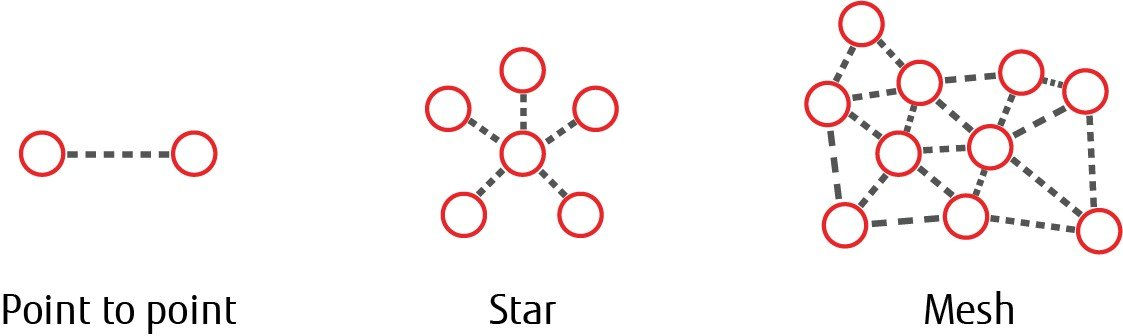
\includegraphics[width=.9\linewidth]{images/network_topologies.jpg}
    \caption{Common IoT network topologies}
    \label{fig:network_topologies}
\end{figure}
  
\subsection{Topologies used in IoT clusters}

All of these topologies can again be organised as flat or segmented. In a flat network all the organizations devices are connected onto the same network. In a segmented one the network is separated into different segments connected by e.g. a router. The segmented solution is preferred from a security aspect as any attack predominantly will be limited to the specific segment. This does on the other hand restrict the agility and feeling of seamlessness within the network.\\

The three topologies mentioned in the previous section are the ones most used in IoT clustering \cite{oreilly:IoT_topology}\cite{linklabs:IoT_topology}. As this project concerns clusters and point-to-point is exclusively between two devices it is natural to take a closer look into the mesh and star topologies.\\ 

Mesh topologies are good for extending networks using short-range protocols like Zigbee and Z-Wave. It is also good if you need bandwidth enough for large data streams. Full mesh is relatively expensive to install, but very fault tolerant in the way all nodes have redundant paths of communication. It allows a high number of nodes in the network, but maintaining all is costly in the form of power consumption. Since a mesh network does not have static routing the timing and latency of the network can vary, making it unfit for time critical applications.\\

From a security aspect mesh topologies are more vulnerable if breached. The moment one relay is breached, all others can be accessed. This vulnerability can be reduced by implementing a part meshed network where only nodes that needs to function as relays will have this privileges. This way e.g. devices like sensors can be attached as leaf nodes. \\

Peter and Perttunen \cite{network_topologies} state that this type of network is most used in military, tactical and other critical applications. This is because of the high degree of reliability, but is also makes the networks more vulnerable, which in turn is more demanding for the remaining security solutions. The consequence of choosing a less ideal network topology is that the remaining security systems potentially need to handle a heavier load. \\

The star topology saves costs where the mesh does not. On the other hand it does not have then same capabilities when it comes to extending the rage of a network since all leaf nodes must be connected to the centre. It is consistent, predictable and fast\cite{oreilly:IoT_topology}.

This makes the star topology an ideal choice if you have a lot of low-level devices like sensors distributed over a confined area. The major drawback of the star topology is that it is reliant on one single gateway. If one of the leaf nodes are attacked the breach is contained within this individual link. If the gateway is breached, an attacker would have full access to the entire network. \\

Topology control is a widely used concept in Wireless Sensor Networks \cite{intrusion_detection}. It is a collection of methods and guidelines on how to cluster IoT applications in a secure way while maintaining integrity, authenticity and reliability. The concept of topology control also mentions network redundancy, which means that it can be useful to deploy a larger number of nodes than what is needed. An increase in nodes increases the attack surface and in turn the vulnerability of the system if the topology control scheme fails.

\subsubsection{Network security threats}
Several scientific articles \cite{electronics:topology_control}\cite{minas_gerais:topology}\cite{intrusion_detection}\cite{IJCSIS:attack_survey} discussing network-topology and control mentions possible attacks related to the networking aspect of an IoT cluster. 

The different attacks has been classified into two groups; one for attacks related to connection to or editing of the nodes composing the cluster. The second for attacks related to normal operations conducted by the network. In Figure \ref{fig:WSN_attacks} below researchers G. Padmavathi and D. Shanmugapriya \cite{IJCSIS:attack_survey} have created a map of possible attacks launched towards Wireless Sensor Networks. As IoT clusters usually contain one or more wireless sensor this is also relevant to this study and several of the attacks will be revisited in the following sections. 

\begin{figure}[h]
    \centering
    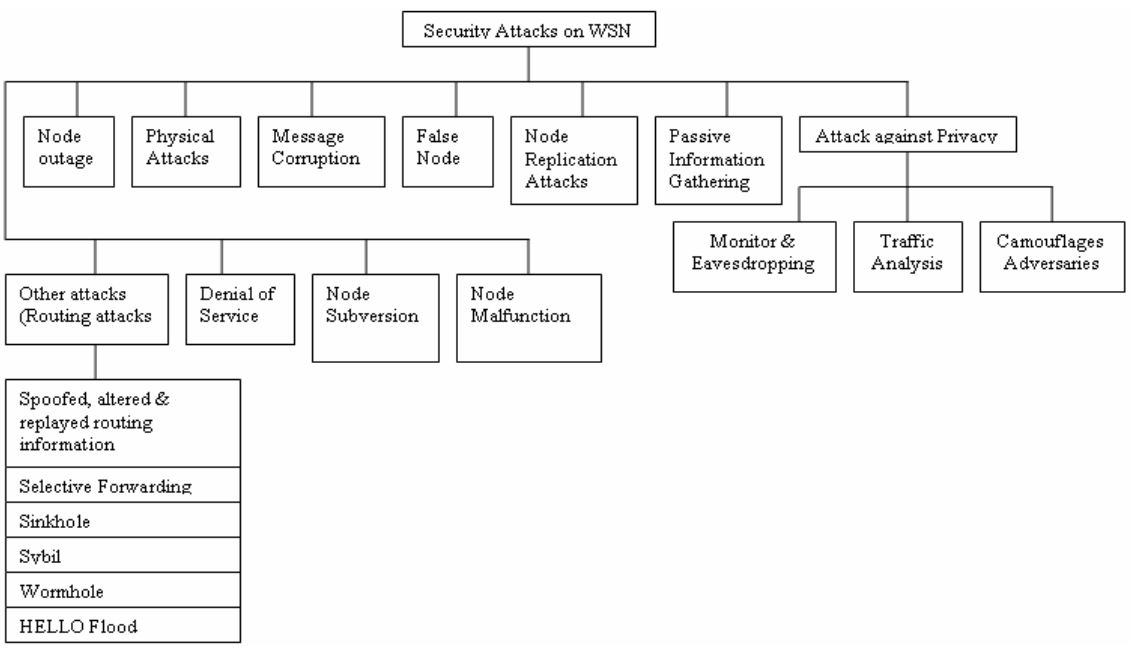
\includegraphics[width=.9\linewidth]{images/attack_classification_WSN.JPG}
    \caption{Classification of possible attacks on WSN \cite{IJCSIS:attack_survey}}
    \label{fig:WSN_attacks}
\end{figure}

\paragraph{Scalability and connectivity} \label{sec:scalability}
An agile network should have the possibility to scale according to user needs. This means adding or removing nodes without necessarily reconfiguring the entire network.

Nodes in different places of the network topology uses different amounts of energy. If a node is used for relay purposes it will use more energy. Because of this the energy signature of a node can be used to decide which nodes should be breached \cite{electronics:topology_control}. Unfortunately it is not possible to monitor if a attacker is monitoring the signature without extra sensors or equipment.

\paragraph{Node subversion} \label{chap:node_tampering}
The attacker steals or tampers with an already existing node in order to steal information or modify transmissions in and out of the node. As the existing node is already connected to the network the cryptographic keys become vulnerable.

\paragraph{False nodes}
An attacker adds a false node to the system in order to obtain information about the network or interrupt transmissions between real nodes. A false node can also be used to conduct a network flooding attack which is similar to a DoS attack where the false node overloads network capacity by flooding the network with useless information. A false node can also be used to conduct a MitM attack. 

\paragraph{Node Replication}
Similar to a false node attack. The attacker replicates the ID of an existing node and impersonates this node to flood the network or inject false information. 

\paragraph{Node outage}
Old or outdated nodes are not an attack in itself but can in worst case be exploited by an attacker to gain access to the rest of the functional network. It can also lead to the node malfunctioning and expose the integrity of the network. 

\paragraph{Routing attacks}
All networks require information to be routed around according to some routing philosophy. The routers in charge of forwarding packets can be attacked in a number of ways \cite{IJCSIS:attack_survey}. 

\begin{itemize}
    \item Spoofed or altered
    \item Selective forwarding
    \item Sinkhole attack
    \item Sybil Attacks
    \item Wormhole attacks
    \item HELLO flood attacks
\end{itemize}

All of these attacks have in common that they affect the network layer and the behaviour of the router is altered to either dismiss or snatch up messages.

\subsubsection{General network attacks}
The following attacks can happen to or between any node. The attacks can be more or less likely depending on the type of protocol used to implement the network topology. 

\paragraph{Eavesdropping}
Snapping up amounts of data traffic to discover the content of messages sent on the network. Also known as sniffing or snooping. 

\paragraph{Traffic analysis}
Analyzing the traffic sent over the network to deduct patterns of usage or other information even if the information is encrypted. 

\paragraph{Denial of Service} 
In a DoS attack the attacker exhausts the networks resources by sending spam data and thus prevents real nodes from sending their data. DoS attacks can again be divided into authentication request flooding, Association request flooding, Rouge Spoofing, CTS/RTS and injection of malicious packets \cite{intrusion_detection}. A DoS attack can lead to network failure which in turn leads to a disconnected system. Jamming is a type of DoS attack which prevents nodes from communicating by completely occupying a channel or port. 


\paragraph{Normal operation states}
As discussed in Section \ref{sec:scalability}, changes in network topology are normal operations. At the same time many attacks are also connected to these types of activities. This makes it natural to monitor operations like addition, removal and reconnection of nodes. 

There is also a rage of attacks targeting routers. In these attacks the routing stream of packages is altered from the natural created by a routing algorithm. If a routing algorithm works correctly it should distribute traffic evenly or at least avoid any router from exceeding bandwidth capacity. In this case the load on each router should be monitored and compared.

 
\paragraph{Attack signatures}
Some attacks uses methods that are easily recongnized and can be classified as attack signatures. The group of attacks included in Denial of Service all have in common that a large increase in packets or requests are injected into the network. For this type of attacks it could be useful to monitor all occurrences where a high frequency of packets or requests are detected on the input port of a node.  \\

A Man in the Middle attack is more difficult to detect but a normal approach is to monitor changes in RTT of packets sent between nodes, as this is likely to increase during a MitM attack. This is on the other hand pointless if the implemented topology is mesh where routing is dynamic. The strength of the transmission signal is also likely to decrease since an attack often is conducted further away than the location of the device. This again only works when the distance between the communicating nodes is fixed. \\

To avoid an attacker from exploiting outaged nodes production date or performance indices of nodes should be monitored to ensure they do not exceed some threshold. This is not specifically an attack signature, but it is a signature that can be used as a preventive asset. 













\section{IoT communication protocols}

IoT devices come in all shapes and sizes and used in a wide range of applications, but they share one common main goal, to collect and transmit data. Communication can either be wired or wireless, where the main concern for this kind of smart devices is the latter. Since there is no unique standard, multiple communication protocols are in use, depending on the requirements, such as, the data bandwidth, the radio range, the power consumption, the  topology or the security constraints. \\

This section will describe the main protocols used in IoT communications, as well as the advantages and disadvantages between them. Typically, the type of connectivity is given by the distance the data must travel, in such scenario, it is possible to divide the most common network protocols in two categories: \textit{Low-power, wide-area networks (LPWAN)} and \textit{Low-power, short-range networks} \cite{Microsoft:protocols}. The classification diagram is shown in figure \ref{fig:NetworkClassification}.


\begin{figure}[h]
    \centering
    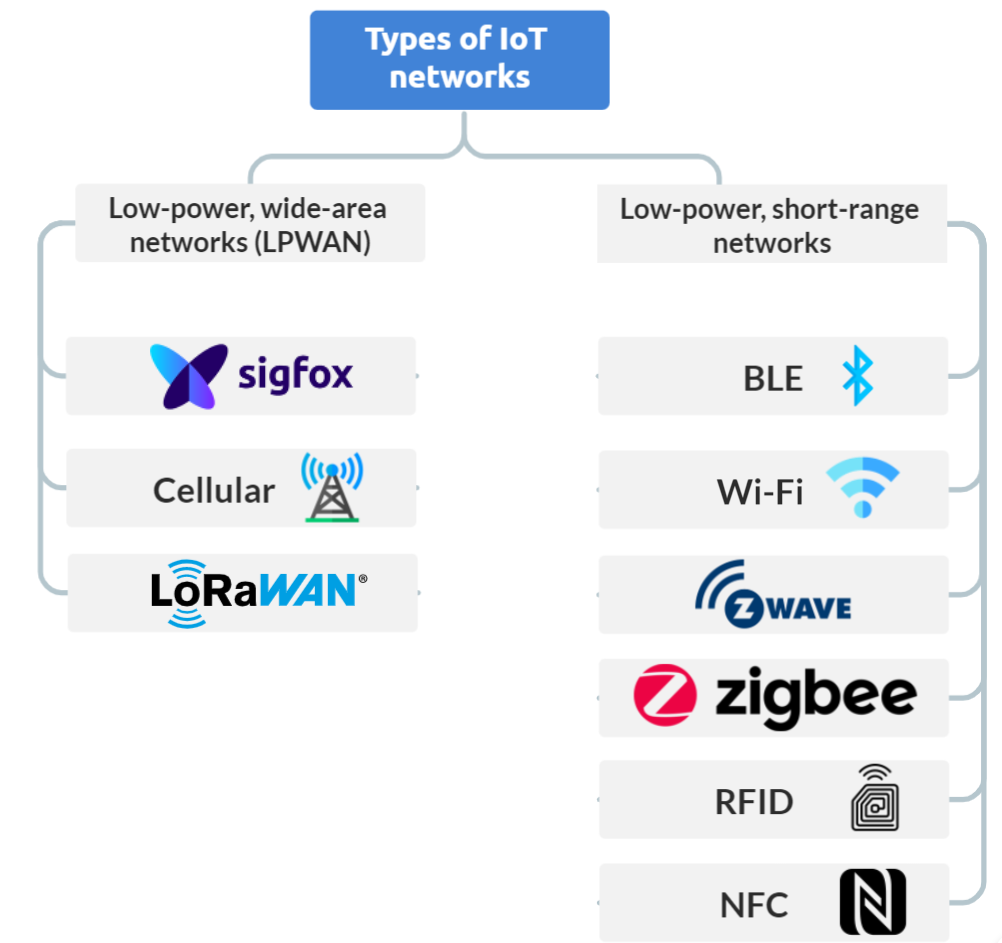
\includegraphics[width=.9\linewidth]{images/TypeOfNetworks.png}
    \caption{IoT network classification}
    \label{fig:NetworkClassification}
\end{figure}


\subsection{Low-power, wide-area networks (LPWAN)}
The main characteristic of LPWANs is to provide long-range communication on low-power devices. These protocols are better suited for applications that do not require high bandwidth or time-sensitive constraints \cite{BehrTech:protocols}.

\subsubsection{Sigfox}
The Sigfox technology is intended for Machine-to-Machine (M2M) communication. It uses an Ultra Narrow Band channel, making data transfer speed as low as 10 to 1000 bps. On the other hand, distance between nodes can go up to 50 Km \cite{IEEE:protocols}.

\subsubsection{Cellular}
Although cellular networks are under the LPWAN category, they are not by any means cheap on power, on the contrary they impose high power requirements, but provide high speed communication over long distances, taking advantage of the installed GSM/3G/4G/5G mobile networks. Cellular technology is not viable for most IoT devices, since they are battery-operated.

\subsubsection{LoRaWAN}
The Long-Range Wide-Area Networks (LoRaWAN) is intended for transmitting small size payloads over long distances. Devices supporting this technology are optimized to operate in a low power mode, lasting up to 10 years on a single cell battery. Signals can be sent and received over a distance of 3 km in urban areas or 10 km in rural areas. The network is secured by end-to-end AES-128 encryption \cite{LoRaWAN}.

\subsection{Low-power, short-range networks}
This type of networks are better suited for homes, offices or small environments, since they can support short range communication, with the advantage of being inexpensive to operate and require small batteries.

\subsubsection{Bluetooth Low Energy (BLE)}
BLE is very significant protocol in the IoT world. According to the 2022 market report written by Bluetooth \textregistered, It is estimated that about 35\% of all IoT connected devices rely on this protocol \cite{BLE1}.
BLE was designed for short-range communications with low latency, but with low bandwidth. However it takes into account a very low power consumption. We can find devices relying on this technology in audio streaming devices, PC peripherals, accessories and fitness and health wearables. Nowadays, also very common in asset tracking and indoor navigation where GPS can not be used.

\subsubsection{Wi-Fi} \label{sec:wifi}
Wi-Fi technology is pretty much spread all over, including IoT applications. It provides high-throughput data transfers. However, due to its high imposing energy requirements, WiFi is not a feasible network protocol for IoT running on batteries. Instead, it is more suitable for devices that are connected to the power outlet, as security cameras or smart home appliances. The allowed distance is usually within the range of 35 m indoors and 100 m outdoors \cite{IEEE:protocols2}.

\subsubsection{Z-Wave}
It is a standard designed for remotely controlled residential applications, it can deliver a transmission speed of 40 kbps reaching up to 30 m. It uses AES-128 encryption for securing the channel \cite{IEEE:protocols2}.

\subsubsection{Zigbee}
This protocol is based on the IEEE 802.15.4 standard, it is intended for short-range low-power communications, typically deployed in mesh topologies to extend the coverage. It provides a low bit rate up to 250 kbps. It is possible to connect 65000 nodes in a single zigbee network. Operates in a rage of 10 to 100 meters 

\subsubsection{RFID}
Radio Frequency Identification (RFID) consists of small readers and RF tags transmitting small amount of data through radio waves within very short distances. RF tag are electronically programmed with unique information, so they cannot be used to collect measurements. However, RFID has had a great positive impact in retail and logistics, as tags can be attached to all kind of products for inventory tracking.

\subsubsection{NFC}
Near-Field Communication (NFC) is a protocol very similar to RFID. It can connect two devices in a distance shorter than 4 cm. It can be used for identification (similar to RFID), but also for more capable two-way communication. This technology is now extended to mobile phones, contactless payments and different industrial applications.\\

Table \ref{tab:DiffNetworks} provides a comparison between the different network protocols most used in IoT scenarios \cite{IEEE:protocols}.

\begin{table}[]
\centering
    \resizebox{\textwidth}{!}{\begin{tabular}{lcccc} 
         \hline
         Technology & Range & Data Rate & \makecell{Power \\consumption} & Topology \\ 
         \hline
         Sigfox & \makecell{10 km (urban) \\ 50 km (rural)} & \makecell{100 bps (urban) \\ 600 bps (rural)} & 10 - 100 mW & Star \\ 
         Cellular & Several km & 8Mbps (3G), 50Mbps (4G) & High & -\\ 
         LoRaWAN & 	$<$ 10 km & 27 kbps & High & Start\\
         \hline
         BLE & 15 - 30 m& 1 Mbps & Low (30 mA) & Star-bus\\
         Wi-Fi & $<$ 100 m & $>$ 100 Mbps & High & Start, Mesh \\
         Z-Wave & $<$ 30 m & 40 kbps & Low (2.5 mA) & Mesh \\
         Zigbee & 10 - 100 m & 250 kbps & Low (30 mA) & Star, Mesh\\
         RFID &  200 m& 4 Mbps& Ultra-low & Point-to-Point\\
         NFC & $<$ 4 cm & 106, 212, 424 kbps& 50 mA& Point-to-Point\\
         \hline
    \end{tabular}}
    \caption{Comparison between network protocols}
    \label{tab:DiffNetworks}
\end{table}













\section{FreeRTOS monitoring} \label{chap:freertos}

This project regards IoT clusters where the devices are running the FreeRTOS operating system. This chapter looks closer into the OS itself and how different attacks can be detected in terms of behavioural changes in the system. \\ 

\subsection{FreeRTOS}

The FreeRTOS is a open source real-time OS created for microcontrollers and small microprocessors \cite{manual:freeRTOS}. It is well suited for systems with both soft and hard real-time requirements. Using the kernel allows the programmer to leave timing to the OS, as well as modularity, easier maintainability and several other benefits.\\

The OS implements a real-time kernel in the shape of a scheduler in order to allow different processes to run independently. The scheduler can also exploit several cores to run concurrent processes. In the FreeRTOS a process is called a thread, but it will be reffered to as a process or a task. To be able to schedule the different threads of the system to the right time the OS use priorities. It is pre-emptive, meaning running processes can be interrupted and suspended to allow a process with higher priority to run. The priorities are configured such that a low numerical value corresponds to a low priority task, with zero being the lowest possible priority.\\

Processes can communicate using semaphores; both binary and counting, queues, mutexes and events. The OS is built up by a library of source and header files. There are two distributions of the OS - one providing the bare minimum of functionality and one supporting amongst other several communication protocols. For this project the basic version of the FreeRTOS was examined and is therefore the one referred to here. To build the kernel different source files need to be configured but the standard project requires files.\\

\begin{itemize}
    \item tasks.c
    \item list.c
    \item queue.c
    \item timers.c
    \item event\_groups.c
    \item croutine.c - only if event groups are used
\end{itemize}
 


\subsection{Monitoring to detect attacks} \label{chap:freertos_monitor}

For a keylogger to be effective it must provide the recipient with useful information. This means that the goal must be to monitor both extraordinary events that are not in the normal behavioural pattern of the application and changes in normal behaviour. \\

An important remark is that to be able to provide such useful information knowledge of the specific system and its user patterns is needed. Simply logging all events might not prove useful but will often be connected with a certain threshold or pattern. This is further explained and examplified in Chapter \ref{chap:real_world_app}.  


\subsubsection{Change in memory usage}
If the rate of memory accesses changes drastically over a specified interval this can be a sign that an attacker tries to fill the devices memory. This could be connected to certain areas in memory storing critical data. The attack signature could match a buffer overflow attack, where the attacker purposely write excessive data to a buffer to gain access to the program memory of the device \cite{buffer_overflow}. This type of attack would be closely connected to the hardware and the hardware abstraction layer of the software rather than the OS itself. 

\subsubsection{Scheduling}
A way of launching a DoS attack on an operating system level could be to request the device to launch a series of high-priority tasks resulting in the system starving lower-priority task even if they are necessary to perform. It could also be as simple as launching too many tasks at once. This could be monitored by logging the number of current existing tasks and the priority of the respective tasks. An alternative to the starvation case could also be to measure the time passed after violating a hard real-time task requirement. 

\subsubsection{Communication}
If a node in the network is attacked, a potential next step for the attacker could be to try disable central nodes by launching a another type of DoS attack where the attacker requests connection or other sorts of data. In that case, the frequency of sockets opened in the node could be monitored and if an attack within the node itself is suspected, one could also note the frequency of tasks filling the socket for sending.\\

For rigid IoT clusters the number of nodes are rarely changed and most devices are online for the most of the time. For these cases monitoring the number of open ports and their belonging IP addresses could help detect node subversion and addition of false nodes. 













\section{IoT Attacks and Safety implications}

\subsection{IoT Vulnerabilities}
Since IoT devices have applications in many different fields, each with varying energy and hardware constraints and with different communication methodologies, the attack surface for cybercriminals is very wide. Design of IoT devices needs to carefully examine the potential vulnerabilities and the corresponding protections that need to be implemented.\\
    
To aid in the detection and prevention of attacks, and the development of security systems to protect IoT devices, multiple security principles have been identified by Staddon, E. et al \cite{IoT_categorization}, shown in Figure \ref{fig:security_principles} below. These need to be addressed in the design phase to achieve a secure design.\\

\begin{figure}[h]
    \centering
    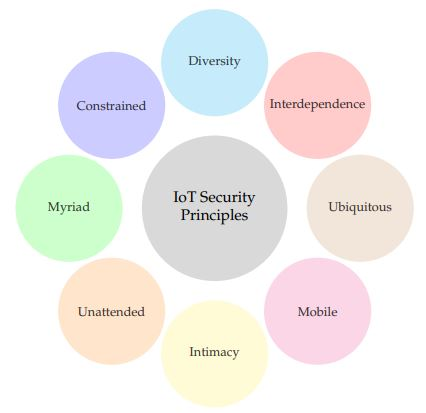
\includegraphics[width=.8\linewidth]{images/IoT security principles.JPG}
    \caption{IoT security principles proposed in the paper}
    \label{fig:security_principles}
\end{figure}

Take for example the Interdependence security principle, it states that since IoT systems are increasingly interconnected, the need for human interaction is diminished and allows for attackers to modify the system's behaviour by interfering with a single device. One real world use case would be a set of smart lightbulbs controlled by a light sensor, if the attackers gained control of the light sensor, they could send some malicious information to turn off the lightbulbs and irrupt into the house undetected.


\subsection{Types of attacks on IoT devices}
The same report by Staddon, E. et al \cite{IoT_categorization} proposes several categorization methods for IoT attacks, including labeling attacks based on the severity of the attack, the attack type or the access type, to name a few.\\

One of the proposals is to divide the attacks into three level related categories, \emph{Low-level}, \emph{Intermediate-level} and \emph{High-level} security issues. Low-level security issues encompasses threats to the lowest network layers, but also to the device's physical state. This includes attacks such as jamming, which disrupts network communication by saturating the communication channel or Denial of Sleep, in which the IoT device is constantly "kept awake" by issuing requests or by other means and this way the battery of the device is drained considerably more rapidly than it normally would. A DoS attack, another type of low-level attack is ARP-Spoofing, where a malicious attacker can access, modify or even stop data-in transit by obtaining a legitimate computer's IP address through malicious Address Resolution Protocol (ARP) messages.\\

Intermediate-level attacks are labeled as those directed against the network and all transport layer related activities, such as a routing and session management. Some examples of Intermediate-level attacks are Replay attacks, where data transmission is maliciously repeated or delayed, or a Sinkhole attack, where a malicious set of nodes modify the network traffic in order to prevent the base node from receiving the correct information.\\

The final High-level attacks are those that target the application itself, they revolve around application vulnerabilities, such as insecure public interfaces, causing a breach to data privacy, or insecure software/firmware, allowing the attacker to take advantage of injection attacks like SQL or XML-injection.\\

It is important to highlight that this is just one of the dozens of categorization methods that exist for cyberattacks on IoT devices. From a security perspective it is interesting to study several categorization methods and offer protection against the types of attacks a specific IoT system might be vulnerable to.\\


\subsection{Safety and security implications of IoT attacks}
Since the attack surface on IoT devices is so big, many different severe consequences can result from a successful IoT cyberattack, we will look at some real world examples to understand the scale of the damage that could be inflicted.
\\~\\
One example would be the exploit of a \hyperlink{https://thehealthcareblog.com/blog/2019/07/29/security-crisis-of-cardiac-pacemakers-paves-the-way-for-iot-security-evolution-in-cardiology/}{vulnerability detected in 475k pacemakers}, this attack would expose critical health parameters of thousands of people that could be manipulated to cause harm/death.
\\~\\
Another IoT system in which attacks could have critical consequences is the smart-cars, which are rising in popularity, and \hyperlink{https://www.lifewire.com/how-self-driving-cars-can-be-hacked-5114337}{many possible attacks have already been proven to exist}, endangering not only the occupants of the car, but also other external actors. 
\\~\\
In general, we can observe that the IoT industry is vulnerable to many different types of attacks with very high damage potential, which is why protection, prevention and detection of these attacks is extremely necessary.



\chapter{Implementation Overview}

\label{chap:real_world_app}

The previous chapters have discussed specific vulnerabilities. To set the theory into a more comprehensible setting the following chapter contains three use cases describing real life applications where IoT clusters can be used. For all of the cases a security assessment is conducted based on the previous discussed theory and a selection of possible parameters to monitor will be suggested.\\ 

IoT applications handle different types of data and have different functionalities. Consequently the data we want to protect differ from one case to another. Therefore it is natural to assume that keyloggers implemented in would have to monitor parameters related to the data we want to protect, or parameters that could indicate that an attacker is trying to exploit a known vulnerability. \\

As previously visited the topology and communication protocol could lead to specific vulnerabilities. The way a user interacts with a device also changes how monitoring and logging should be done effectively. A lot of IoT devices are built on a deterministic design principle and will therefore not have any form of user interaction, like sensors. Some will have limited interaction possibilities like buttons to power on, choose functionality and connect to network, such as household applications. More advanced devices could have a graphical user interface, but these devices are not as relevant for this project as they would use a more powerful OS than the FreeRTOS.\\

Logging user activity could be in the sense of logging the internal processes of the specific device, or it could log the behaviour of other nodes in the network. A combination of both is also possible. Moving on with the assumption that the FreeRTOS will be running on devices with limited or no user interaction, one can draw some conclusions about monitoring. \\

For a deterministic device with no user interaction, monitoring internal processes might just be a waste of resources. Monitoring communication in towards the device, attempts on connection and tampering with real world parameters like power supply would be more meaningful. If the device on the other hand has some extent of user interaction like buttons or a terminal it would be relevant to log user activity like interrupts from button presses. If the device has communication ports these should also be monitored.\\

\section{Health Monitoring} \label{chapter:use_case_1}
When entering the healthcare sector a lot of sensitive data regarding patients needs to be handled. If an outsider gains access to personal health data it could potentially be critical for the patients safety. This specific use case concerns the use of monitoring bracelets on residents in an elderly home. Each resident has their own bracelet monitoring biological parameters such as temperature, heartbeat or insulin levels if the patient has diabetes. 

Each device is connected to a WiFi network. Caretakers have their own devices (gateways) with the capability of receiving data from patient bracelets, which also send the data to an external server to be processed. This particular cluster would be exposed to vulnerabilities of the WiFi protocol, the network topology and general network attacks, as well as attacks on the device's hardware.\\

One surface of attacks can be against the physical devices themselves, in this particular use case, it could lead to the biological parameters of an elderly person not being monitored, with the corresponding danger this entrails. We have identified several possible attacks, the first would be a Denial of Sleep attack caused by, for example, constant data requests by a malicious gateway, preventing the IoT device from entering "sleep" mode in order to save battery. To detect this kind of attack, the device can monitor the amount of data petitions it is receiving, the time it has spent in "idle" mode as well as its remaining battery life. \\ 

Denial of service is a similar attack against the device's hardware, which can compromise its correct functioning by overloading the device's CPU or memory, this can be countered by monitoring the overall CPU/memory usage. Starving the tasks which monitor the patient's vital signs of resources through some attack on the monitoring bracelet's OS could also be a possibility.\\

Side Channel attack like those covered in this course could be taken into consideration, as they would allow the user to manipulate many of the device's parameters through the extraction of, for example, administrator credentials. This would involve the attackers measuring the device's response against different inputs, allowing them to extract confidential information. Detection of side channel attacks require extra equipment.\\

For this specific use case the nodes of the network are mobile, which means the likelihood is high of a node moving into an other part of the network topology or disconnect for shorter time periods. A way of intelligently monitor if a node has been tampered with while disconnected is to check if the network traffic coming from a recently disconnected node has changed, which could indicate it has been subverted. Keeping a whitelist would also be a good tool for this purpose.\\

When the monitoring tasks encounters unexpected values in any of the parameters that are monitored, it will raise an alarm to be broadcasted to the gateway.


\section{Oil Platform Control Systems}

Oil rigs are highly safety critical installations. If attacked and shut down the environment around can suffer great consequences. To operate a rig several different WSNs are used both separately and collectively. Therefore a suitable network topology could be a part mesh topology where the sensor units themselves only transmits to dedicated relay nodes. The Zigbee protocol has an operating range of 10 - 100 meters which is realistic for the proportions of an oil rig. The network would also be extended end-to-end by the mesh topology. \\

Both offshore and onshore rigs could be victims of node tampering and internal network attacks. According to Siemens Energy\cite{cyber-attacks_oil} attackers are no longer satisfied by injecting malware into the IT systems, but are starting to attack the OT systems of the business. If the control systems of an oil platform is attacked it could lead to failures like overheating, leakages or inability to detect broken parts or systems. \\

From the previous reasoning types of attack that disable or surrenders critical systems in favour of the attacker seems the most relevant. This could be the addition of malicious nodes or node subversion, like mentioned in Chapter \ref{chap:node_tampering}. This could be detected using a keylogger monitoring the addition of unknown nodes or reappearance of seemingly disconnected nodes. In this use case all such events could be reported as the changes of sensors or other control devices is likely to be well planned and scheduled by trained operators. In addition such systems have strict requirements about connectivity and are required to be online at all times. That would make it easy to filter out any false positives.\\

A WSN like this could be composed of different types of devices as discussed in the introduction of this chapter. Central nodes responsible for network administration and relaying are more likely to have user interaction so monitoring both interrupt handling and user inputs could detect if someone is trying to launch an attack from the node. Node administration on a socket level is also relevant if node subversion is conducted or false nodes are added to the network.\\

If a node has been breached there is a possibility that the attacker will try to launch a DoS attack to disable central nodes in the network. In that case parameters like frequency of sockets opened and high-priority tasks launched should be monitored like discussed in Chapter \ref{chap:freertos_monitor}. 

\section{Security Cameras}

Surveillance cameras are tools used for obtaining safety, but when compromized create vulnerabilities. Surveillance cameras are as described in Chapter \ref{sec:wifi} often stationary and connected to the Wi-Fi. In a realistic use case the cameras would be stationed around a building and transfer data to a hub or server. This makes the star topology a suitable choice for this application.\\

In this use case we have the same situation as the last where nodes rarely are added or replaced. In addition all cameras should only be connected to the master device, all other attempts of connection would be an abnormality unless the whole system is being reconfigured. On the other hand security cameras are more likely to be connected to a commercially internet service provider which might not deliver the same reliability as for industrial purposes. Thus drawing the conclusion that nodes going offline and then reappearing may not be a sign of an ongoing attack. However, a disconnection and then reappearance of an unknown could be a sign that something is not as it should be.\\ 

For a device with the purpose of monitoring, like a security camera, an attacker could be interested in tapping into the stream of information rater than damage the device. That makes attacks like eavesdropping, traffic analysis and MitM relevant. However, these types of attack are rather hard to monitor and detect. For a MitM attack a possibility is to monitor the transmission power of a signal and the RTT of communication. \\

In terms of possibilities of logging operating system variables the attacks monitoring network traffic is rather hard, but monitoring open sockets with belonging IP-addresses and cross-check it against an inventory list could be a good choice.  


\chapter{Use Case Implementation}

The project includes a demonstration of Use Case 1 from Chapter \ref{chapter:use_case_1}. The implementation has been done on several ESP32 board running FreeRTOS which are both described in Chapter \ref{chap:freertos}. The keylogger application is built and deployed on one of the ESP's dual cores. The other one is used to fulfill the specifications of the use case. \\

The keylogger application was built using the ESP-IDF with resources from the FreeRTOS documentation and the ESP-IDF example projects, as well as other projects that can be found online. All the code that is discussed in this segment can be found in the project's \href{https://github.com/C4ES-PoliTO/FreeRTOS-Monitoring}{\textbf{github repository}}.

\section{ESP-IDF}
This project deploys as previously mentioned FreeRTOS on an ESP32 board \cite{manual:ESP-IDF}. The Espressif IoT Development Framework is a development environment containing build tools and \hyperlink{https://github.com/espressif/esp-idf/tree/master/examples}{\textbf{example projects}} as extensions for the Visual Studio Code and Eclipse IDEs. 

These resources can be used on top of the minimal version of FreeRTOS to support several communication protocols, tracing and other functionalities useful for a keylogger.

\section{Network topology}
As is described in the Use Case 1, we are dealing with a set of patients carrying the monitoring devices, they form a star topology together with a gateway, which can be either carried by a nurse or fixed in a given location. In order to achieve a robust connection and to facilitate the collection of network parameters and traffic, we have set up the central node to work as an Access Point and create a Wi-fi network which the patients connect to. More information on monitoring the network traffic will be provided in the section \ref{sec:CentralNodeMonitoring}

\begin{figure}[h]
    \centering
    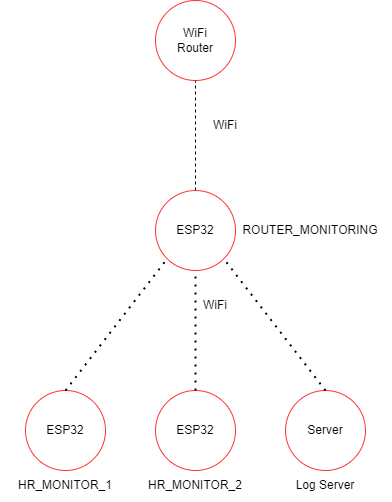
\includegraphics[scale=0.5]{images/uc_topology.png}
    \caption{Network topology of use case 1.}
    \label{fig:uc1}
\end{figure}


\section{Monitoring the devices}
Firstly, we have undergone a process of transforming the user requirements (Use case specifications) into technical objectives set for development. When studying the architecture of the ESP32 in this solution, we can see that it offers a very attractive feature in terms of monitoring capabilities: A dual core.\\ 

This dual core enables a user application to be deployed in the first core (Core 0), supported by FreeRTOS. The \textbf{monitoring tasks} deployed on the second core (Core 1) focus on "spying" on the application to collect different kinds of data and extract vital information from it. One example of this is our monitoring task can check what sockets are being used at any given time, collect the IPs and examine whether the device is communicating with an unexpected source.
\\~\\
Now we will cover the implementation of the different monitoring techniques that have been applied to both the leaf nodes and the central node in our IoT solution.


\subsection{Code Structure}
As a preface, it is important to remark that the code is divided in two main segments, contained in the "Source\_code" folder of the github repository. The first contains all aspects of the leaf node. The (esp32\_leaf\_node) folder is built and flashed onto the ESP32 that act as the leaf nodes.
\\~\\
The second segment is the one contained in the folder "esp32\_nat\_router", this one is built and flashed onto the esp32 which acts as the central router.
\\~\\
Another approach would have been to merge the codes and have some kind of variable similar to IS\_LEAF\_NODE which determined the program flow to follow, but due to development, readability and reusability concerns we have decided to separate and modularize the code in this form.


\subsection{Leaf node monitoring}
In this use case, the leaf nodes measure vital information from the patients, then sends it to the gateway to be transferred to a server which makes sure all the patients are at good health.
\\~\\
However, we have aimed to abstract the use case and offer a monitoring solution that can be easily implemented in any other use case and still provide valuable information.
\\~\\
When designing the monitoring functions for the leaf node, there are several interesting parameters than can give us important information about how the system is behaving. When researching attacks it was discovered that launching a large number of tasks to be scheduled can become overwhelming for the operative system. This can produce a denial of service attack, especially if the attacker finds a way to launch high-priority tasks that can starve lower priority functionality. The possibility of launching low-priority task to starve high-priority ones could have produced more severe results. However, this is avoided by the priority inheritance feature that is implemented in the operative system in order to avoid priority inversion. \\

Therefore, it was natural to implement a functionality that monitors the number of tasks created within a time interval and use this data to decide whether this could be a potential attack or not. The implementation is based on example code from the ESP-IDF and FreeRTOS API guides \cite{uxTaskGetSystemState} where the vTaskGetRunTimeStats function is used to retrieve real time information about the tasks running on the CPU at a specific moment in time. The information extracted represents the task handle, task name, task priority, task state, and total amount of run time consumed by the task. By probing this at different points in time one can list which tasks have been created or deleted during the last interval in time. \\

All of this information can be sent to the server. Another possibility, which is the intelligent part of the monitoring, is to check the number of created tasks up against some predetermined threshold. It would be the maximum number of tasks to be expected during normal operation. If a node is experiencing an increase in tasks higher than the threshold it sends a message containing the number of created tasks, the number of expected tasks and a list of all the tasks that has been created along with their priorities to also detect potential starvation.\\

\begin{lstlisting}[
  breaklines,
  rulecolor=\color{black},
  frame=single,
  language=C,
  basicstyle=\ttfamily\small
]
void DoS_Monitoring(TaskStatus_t *pxTaskStatusArray, UBaseType_t array_size, int buffer_length, char *writeBuffer, int count) {
    buffer_length += snprintf( writeBuffer + buffer_length, TASK_BUFFER_SIZE - buffer_length,"| DoS suspected, number of created tasks: %u\n", count);
    buffer_length += snprintf( writeBuffer + buffer_length, TASK_BUFFER_SIZE - buffer_length,"| Maximum number of task expected for period: %u\n", THRESHOLD);
    buffer_length += snprintf( writeBuffer + buffer_length, TASK_BUFFER_SIZE - buffer_length,"| Task name | Task base priority \n");
    
    ESP_LOGI(TAG,"DoS suspected, number of created tasks: %d, threshold: %d", count, THRESHOLD);
    
    for (int i = 0; i < array_size; i++) {
        if (pxTaskStatusArray[i].xHandle != NULL) {
            buffer_length += snprintf( writeBuffer + buffer_length, TASK_BUFFER_SIZE - buffer_length,"| %s | %u \n", 
                                    pxTaskStatusArray[i].pcTaskName, 
                                    pxTaskStatusArray[i].uxBasePriority);
        }
    }
}
\end{lstlisting}



This would of course require some knowledge about the application and the normal amount of coexisting tasks. Therefore there are two versions on this monitor - one that outputs all running tasks with belonging information at each time interval, and one that only notifies the network if abnormal amounts of tasks are created.\\

To test the functionality a simple function is run as a part of the testing. This function creates a number of tasks that exceeds the threshold. This triggers the monitor to notify the network. \\


\begin{lstlisting}[
  breaklines,
  rulecolor=\color{black},
  frame=single,
  language=C,
  basicstyle=\ttfamily\small
]
void DoSTask(void * param) {
    int *num1 = param;
    int num = num1;

    while(1) {
        vTaskDelay(pdMS_TO_TICKS(5600));
    }
}

void DoSTest(void) {

    ESP_LOGI(TAG,"DoS test initiated.");

    for(int i = 0; i < THRESHOLD +1; i++) {
        int y = i;
        xTaskCreatePinnedToCore(DoSTask, "DoS test", 4096, y, 3, NULL, 0);
        vTaskDelay(pdMS_TO_TICKS(500));
    }
}
\end{lstlisting}

This monitoring functionality is also added to the central node. The only adaptation that needs to be made is altering the threshold to match the expected number of tasks for this type of node.

The CPU usage of a task can be included to see if the task is receiving inputs that leads it to use abnormal amounts of capacity. This is on the other hand very application dependent, but it could in future implementation check for abnormal portions of capacity. 

\subsection{Socket monitoring}
As part of the leaf monitoring, it is really important to log the network traffic at the device. Specifically, logging the metadata is fundamental, as it provides the destination IP/port, and the size of the message. Since this use case considers a deterministic scenario, all network destinations and sources, as well as the data size range are known in advance. If the log does not match the whitelisted IPs, it is easy to recognize that data is being leaked. In the same way, if the size of the message is much bigger than expected, it could mean that a DoS attack is in process.\\

In order to be able to log all network traffic, independently from the application level, we must resort to the device's sockets. ESP-IDF's network stack relies on the LWIP library, therefore, by modifying the lwip/sockets.c functions it is possible to access to this information, both for UDP and TCP packets.\\

The following functions have been duplicated and modified to log and send the message's metadata to a remote server where it can be analyzed. 
\begin{itemize}
    \item lwip\_recvfrom()
    \item lwip\_send()
    \item lwip\_sendto()
\end{itemize}
Since we do not want to monitor the messages sent by this monitoring task, as it would create an infinite loop, the original functions are also kept, but with a different name, and used only by the monitoring task. Here is an example of the added functionality to the lwip\_send() function. The data is extracted by the corresponding structures, and then sent to UDP server by the created udp\_send\_msg(). 
\begin{lstlisting}[
  breaklines,
  rulecolor=\color{black},
  frame=single,
  language=C,
  basicstyle=\ttfamily\small
]
    ip_addr_t addr;
    u16_t port;
    netconn_peer(sock->conn, &addr, &port);
    char msg_data[1024];
    sprintf(msg_data, "(%s) TCP connection to Socket: %d, IP: %s, Port 
    udp_send_msg(UDP_SERVER_IP, UDP_SERVER_PORT, msg_data);
\end{lstlisting}


\subsection{Central node monitoring} \label{sec:CentralNodeMonitoring}
Another "level" which offers very valuable information is the network, in this regard, we have designed some monitoring tasks that, while not completely application independent, offer a high degree of reusability and portability into other solutions similar to ours.
\\~\\
To fully leverage all the network monitoring capabilities, we have decided for our central node to act as an \textbf{access point} to the rest of nodes, which will connect to it. The node will be then in charge or relaying the information to an external server, in essence acting as a more "intelligent" router. To aid in the implementation of this code, which is not the objective of this project, we have used some code present in \href{https://github.com/martin-ger/esp32_nat_router}{\textbf{this github repository}}, while other resources have been learned through the study of several examples present in \href{https://github.com/espressif/esp-idf/tree/master/examples}{\textbf{Espressif's example projects}}, mainly "SoftAP".
\\~\\
Since we are aiming for an abstraction from the application level, we will not consider the content of the messages or their recipients, though this would also be valid information (And they are partially covered by socket monitoring in the leaf nodes), in fact we will not consider the messages at all, the only parameters we will consider are:

\begin{itemize}
    \item Number of connected stations
    \item MAC addresses of stations
\end{itemize}


Let us analyze these parameters and why they might be interesting from a security point of view. In most use cases related to the one we have based ourselves upon, the number of connected nodes will be relatively stable throughout defined periods of time, therefore if any anomalies in the number of connected nodes is detected, it is very important to relay this to an external server. A bigger than expected number of nodes can indicate that malicious nodes are present in our system, with the ensuing risk, on the other hand, a number of connected nodes smaller than the expected might mean that we have suffered a DoS attack on a number of them, or that our central node has been compromised.\\~\\

The other parameter we are monitoring is the MAC address of our connected devices, the monitoring task has a list of whitelisted MAC addresses, if a MAC address not in this list connects to the wifi, an alarm is sent to the server.\\~\\

The script in charge of monitoring these parameters is \textbf{router\_monitoring.c}, located inside the "main" folder of "esp32\_nat\_router". A FreeRTOS task is created in the main code, linking this task to Core 1. The task first defines an event handler for the event type \href{https://docs.espressif.com/projects/esp-idf/en/latest/esp32/api-reference/system/esp_event.html}{\textbf{system\_event\_base\_t}} which can bee seen in Figure \ref{fig:wifi_event_handler}. 

\begin{figure}[H]
\centering
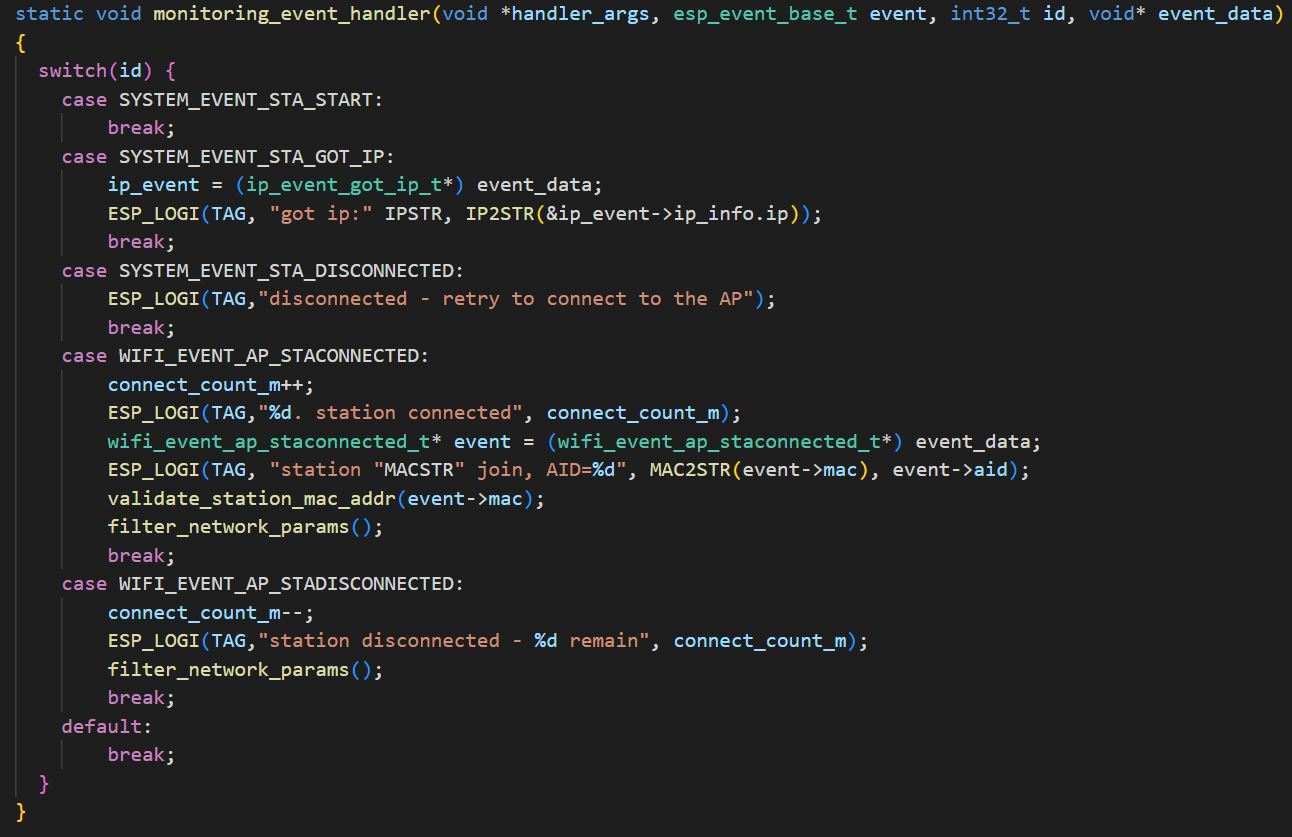
\includegraphics[width=.9\linewidth]{images/wifi_event_handler_code.JPG}
\caption{Wifi event handler code in routerMonitorin.c}
\label{fig:wifi_event_handler}
\end{figure}

This handler is then posted to the \href{https://docs.espressif.com/projects/esp-idf/en/latest/esp32/api-reference/system/esp_event.html}{\textbf{default system event loop}}, which allows the event handler to handle the incoming events, the events we will react to are:

\begin{itemize}
    \item \textbf{WIFI\_EVENT\_AP\_STACONNECTED: } This event is posted to the event loop when a station connects to our Access Point, our monitoring task then checks that its MAC address is whitelisted, if it is not an alarm is raised to the server. The handler also calls \textbf{filter\_network\_params()}, which keeps track of the number of connected stations and checks that it is whithin an expected range, if this is not met an alarm is sent to the server.
    
    \item \textbf{WIFI\_EVENT\_AP\_STADISCONNECTED: } This event is posted to the event loop when a station disconnects, the handler then calls \textbf{filter\_network\_params()} to check that the number of connected stations is in an expected range.
    
\end{itemize}

If any anomalies described above are detected, the monitoring task opens a udp socket to communicate with the monitoring server which receives the alerts.

\begin{figure}[H]
\centering
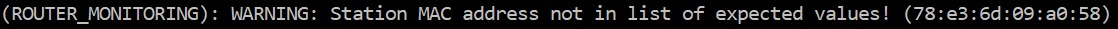
\includegraphics[width=.9\linewidth]{images/monitoring_warning_mac_whitelist.jpeg}
\caption{Alert message recieved by the server when an unexpected MAC addr connects}
\label{fig:monitoring_alert_mac}
\end{figure}

\begin{figure}[H]
\centering
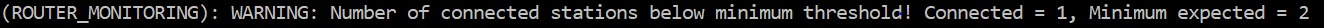
\includegraphics[width=.9\linewidth]{images/monitoring_warning_minimum_stations.jpeg}
\caption{Alert message recieved by the server when too few stations are connected}
\label{fig:monitoring_alert_few_stas}
\end{figure}

\begin{figure}[H]
\centering
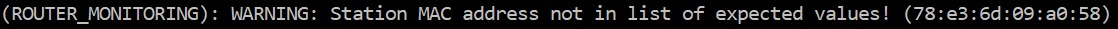
\includegraphics[width=.9\linewidth]{images/monitoring_warning_mac_whitelist.jpeg}
\caption{Alert message recieved by the server when too many stations are connected}
\label{fig:monitoring_alert_many_stas}
\end{figure}
\chapter{Results}
The initial research showed that the variety of attacks that can be launched towards IoT clusters are very diverse and depending on a variety of factors such as communication protocol, topology and system specifications. 

These attacks can be detected in different ways. The background knowledge about the different attacks was used to discover which parameters that are useful when monitoring the FreeRTOS system. 

To monitor DoS attacks the change rate of task creation is useful as well as the priority of the tasks created. The network traffic is also monitored in relation to DoS as well as the size of network packets to see if an attacker is trying to overfill the receiving nodes buffer. To monitor false or subverted nodes the connections with belonging MAC addresses are logged. 

The implementation includes three different monitoring functions. For the leaf nodes the network traffic and tasks are monitored. The same goes for the central nodes of the network, but in addition these nodes monitor connections to the network. The implementation of these three features was successful. 

\section{Known Issues}
Some issues present in the project are the difficulty of modifying certain parameters, for example the monitoring server destination IP address, making it hard for the user to alter the default behaviour of the system, as they need to change the code, compile and build it and flash into the ESP32 development boards.\\

The alert messages from the monitoring server could provide information in a more visually appealing way to the user.


\section{Future Work}
Some further work could be dedicated to eliminating duplicated dependencies and other resources, which take up space in the limited ESP32 memory, as well as induce mistakes.

For future development other parameters could be monitored or existing notifications can be altered to represent information in a more useful way. 

Possible parameters to monitor could be:
\begin{itemize}
    \item Memory allocation
    \item Overloading or emptying of thread synchronization methods
\end{itemize}
\chapter{Conclusions}

In conclusion, this project has given insight into the IoT cybersecurity environment, the study started off looking into how network topologies and protocols affect the different IoT solutions, their vulnerabilities and the scenarios in which they should be utilized to fully capture the benefits they offer.\\

A thorough study of possible cyberattacks on IoT devices has been conducted, together with the implications they would have. The goal has been to understand the security principles that help engineers address and mitigate these attacks which, if left unchecked, could cause devastating damage. During the implementation phase the possibility of achieving this goal using monitoring of the devices and network for anomalous activity has been tested.\\

Several theoretical use cases have been proposed in the paper in order for the reader to understand in which real world scenarios these technologies could prove useful, in them possible cyberattacks, their associated risks and proposed monitoring solutions are explained.\\

Using the FreeRTOS to implement a prototype to monitor one of these use cases proved rather cumbersome. It is quite easy if one know all the system specifications, hardware and circumstances. On the other hand trying to generalize the prototype for portability is the difficult. Mostly because the implementation of a IoT system is in general not portable across systems. This would in most cases require the monitor to be adapted to specific variables. \\

The ordinary version of FreeRTOS contains the minimum required functionality, so both the node connection monitor and the networking monitor utilize additional APIs from the ESP-IDF. Only the task monitor is implemented purely using the FreeRTOS functionality. \\

It is in other words possible to create a monitor using solely the FreeRTOS in order to provide intelligent information about a potential attack. However, the number of parameters that can be monitored without using external resources are limited. Because of this a monitor basing itself on the FreeRTOS core, but also uses some external resources would prove more useful. \\

In conclusion, this project has served to develop a deep understanding of the IoT security environment, the different IoT system configuration, the possible attacks that they are exposed to, the criticality of these threats as well as a way to mitigate and detect these attacks.
\printbibliography[heading=bibintoc,title={Bibliography}]

%%%%%%%%%%%%%%%%%%%%%%%%%%%%%%%%%%%%%%%%%%%%%%%%%%%%%
    
% HERE IS WHERE YOU INCLUDE YOUR APPENDICES (IF ANY)

\appendix
\chapter{User guide}

\section{Setting up ESP32 toolkit}

This is the guide to install all the necessary software to execute the FreeRTOS IoT monitoring demo found in the repository: https://github.com/C4ES-PoliTO/FreeRTOS-Monitoring
\\~\\
This installation guide is meant to be followed using a \href{https://docs.espressif.com/projects/esp-idf/en/latest/esp32/get-started/linux-macos-setup.html}{\textbf{Linux}} operating system (Ubuntu or Debian), for information on running on other operating systems, take a look at: \href{https://docs.espressif.com/projects/esp-idf/en/latest/esp32/get-started/windows-setup.html}{\textbf{Windows}} , \href{https://docs.espressif.com/projects/esp-idf/en/latest/esp32/get-started/linux-macos-setup.html}{\textbf{MacOS}}.
\\~\\
\textbf{Setting up the ESP32 environment:}
\\
\begin{itemize}
    \item Command to install the required packages:
    \begin{verbatim}
    sudo apt-get install git wget flex bison gperf python3 python3-venv cmake 
    ninja-build ccache libffi-dev libssl-dev dfu-util libusb-1.0-0
    \end{verbatim}

    Note: cmake version 3.5 or higher is required, to check the version run: cmake --version
    
    \item Proceed by cloning the software libraries provided by ESP-IDF repository, to do this, create a parent folder and run:
    \begin{verbatim}
    mkdir -p ~/esp
    cd ~/esp
    git clone -b v4.4.1 --recursive https://github.com/espressif/esp-idf.git
    \end{verbatim}

    
    
    \item Update python:
    \begin{verbatim}
    sudo apt update
    sudo apt install python3
    sudo apt-get install python3-venv
    sudo apt intall pip
    \end{verbatim}


    \item Aside from the ESP-IDF, you also need to install the tools used by ESP-IDF, such as the compiler, debugger, Python packages, etc, for projects supporting ESP32:
    \begin{verbatim}
    cd ~/esp/esp-idf
    ./install.sh esp32
    \end{verbatim}

    
    \item The installed tools are not yet added to the PATH environment variable. To make the tools usable from the command line, some environment variables must be set. ESP-IDF provides another script which does that.\\
    
    In the terminal where you are going to use ESP-IDF, run:
    \begin{verbatim}
    . $HOME/esp/esp-idf/export.sh 
    \end{verbatim}
    
    Note the space between the leading dot and the path!

\end{itemize}

\textbf{Running an ESP32 project:}

\begin{itemize}
    \item Clone project files 
    \begin{verbatim}
    cd ~
    git clone https://github.com/C4ES-PoliTO/FreeRTOS-Monitoring.git
    \end{verbatim}

    
    \item \textbf{Navigate} to the project directory, set ESP32 and run the project configuration utility menuconfig:
    \begin{verbatim}
    cd FreeRTOS-Monitoring/Source_code/esp32_leaf_node
    idf.py set-target esp32
    idf.py menuconfig
    menuconfig->Component config->FreeRTOS->Enable FreeRTOS trace facility
    menuconfig->Example Configuration Connection >WiFi SSID  
    menuconfig->Example Configuration Connection >WiFi Password
    \end{verbatim}

    Trace facibility for FreeRTOS needs to be enabled, set WiFi credentials, for the leaf node, use the ones provided by the gateway.\\
    
    After opening a new project, you should first \textbf{set the target}. Note that existing builds and configurations in the project, if any, will be cleared and initialized in this process. The target may be saved in the environment variable to skip this step at all.
    
    \item \textbf{To build the project:}
    \begin{verbatim}
    idf.py build
    \end{verbatim}

    If there are no errors, the build will finish by generating the firmware binary .bin files.

    \item \textbf{Flash} the binaries that you just built (bootloader.bin, partition-table.bin and project.bin) onto your ESP32 board by running:
    \begin{verbatim}
        idf.py -p PORT [-b BAUD] flash
    \end{verbatim}
    
    Replace PORT with your ESP32 board’s serial port name. Similar to /dev/ttyXXX

    Note: For ESP32 board, you will need to press the BOOT button on the board after executing the previous command.\\
    
    If there are no issues by the end of the flash process, the board will reboot and start up the “project.bin” application.
    If you’d like to use the Eclipse or VS Code IDE instead of running idf.py, check out the \hyperlink{https://docs.espressif.com/projects/esp-idf/en/latest/esp32/get-started/eclipse-setup.html}{Eclipse guide}, \hyperlink{https://docs.espressif.com/projects/esp-idf/en/latest/esp32/get-started/vscode-setup.html}{VS Code guide}.\\
    
    \item \textbf{Monitor the output:}\\
    To check if “project” is indeed running, type idf.py -p PORT monitor (Do not forget to replace PORT with your serial port name).
    
\end{itemize}

The instructions that are explained in this document are also available \hyperlink{https://docs.espressif.com/projects/esp-idf/en/latest/esp32/get-started/linux-macos-setup.html}{\textbf{here}}, where more information can be found, regarding different errors or suggestions that are interesting for the correct installation of the esp32 development kit. 

\section{Configuring demo}

Several parameters can be configured in the demo project, the user can choose to modify these to alter the system's behaviour.

\subsection{Central node}

\begin{figure}[H]
\centering
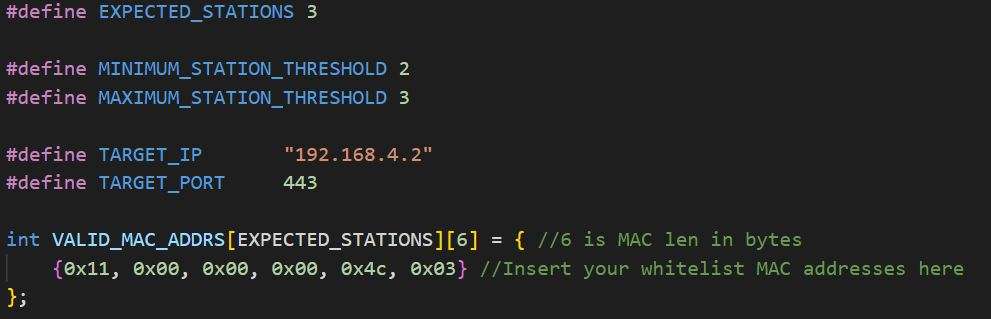
\includegraphics[width=.9\linewidth]{images/router_monitoring_params.JPG}
\caption{Parameters found in "router\_monitoring.h"}
\label{fig:router_monitoring_params}
\end{figure}

In figure \ref{fig:router_monitoring_params} we can observe the parameters that alter the behaviour of the monitoring behaviour, these are the number of expected stations, the minimum and maximum thresholds to alert the server, the IP and Port of the server that will collect the info and the whitelisted MAC addresses.
\\~\\
By default, the Wi-Fi network created by the central node is called "ESP32\_NAT\_Router" and has no password, this can be changed following the steps described \hyperlink{https://github.com/martin-ger/esp32_nat_router}{here}.

The following configuration must be done on the menuconfig

\begin{verbatim}
    menuconfig > Serial Flash Config > Flash size > 4Mb
\end{verbatim}


\subsection{Leaf node}
The leaf node offers two different configuration aspects, the first can be found in the file "sdkconfig" inside the leaf node folder, there the user can change the \textbf{CONFIG\_EXAMPLE\_WIFI\_SSID} and the \textbf{CONFIG\_EXAMPLE\_WIFI\_PASSWORD} to correspond to the ones in the central node configuration.
\\~\\
The other parameters are related to the monitoring task, and can be found in the file "taskMonitor.h". They are; the number of tasks threshold to raise an alert, the task monitoring priority and the monitoring task id which the server will recieve.



\subsection{Monitoring server}
To launch the monitoring server "upd\_server.py" found in both "esp32\_nat\_router" and "esp32\_leaf\_node" the user needs to simply navigate to any of these folders and execute the following command in the Windows/Linux terminals:

\begin{verbatim}
    python udp_server.py
\end{verbatim}

Then the server will start outputting to the console the messages that it receives.




%%%%%%%%%%%%%%%%%%%%%%%%%%%%%%%%%%%%%%%%%%%%%%%%%%%%%


\end{document}